\section{Evaluation Methodology}
\label{sec:evaluation-methodology}

\fxfatal{Evaluation Methodology}

In the previous chapter the field of information extraction was presented. The process of IE does not only require the extraction itself, but also the relevance of localized facts for the respective domain. Thus, a quality assessment is required, which focuses on the advancement of development and the juxtaposition of approaches. The evaluation is the formulation of new problems which have to be integrated into the development \cite{Linsmayr:2010}. The methodology of the evaluation is described in this chapter.

\subsection{Performance measures}
\fxfatal{Measures...}
Core (Precision, Recall, F-Measure) and additional...

For classification tasks, the terms true positives, true negatives, false positives, and false negatives (see also Type I and type II errors) compare the results of the classifier under test with trusted external judgments. The terms positive and negative refer to the classifier's prediction (sometimes known as the expectation), and the terms true and false refer to whether that prediction corresponds to the external judgment (sometimes known as the observation). This is illustrated by the table below \cite{Wikipedia:Precision_and_recall}:

\begin{table}[H]
\centering
\begin{tabular}{cccc}
	& \multicolumn{2}{c}{\shortstack{\textbf{Actual class} \\ (Observation)}} \\
	\multirow{6}{*}{\shortstack{\textbf{Predicted class} \\ (Expectation)}} & \textbf{\textit{tp}}  & \cellcolor{gray!15} \textbf{\textit{fp}} \\
	& (true positive) & \cellcolor{gray!15} (false positive) \\
	& Correct result & \cellcolor{gray!15} Unexpected result \\
	& \cellcolor{gray!15} \textbf{\textit{fn}} & \textbf{\textit{tn}} \\
	& \cellcolor{gray!15} (false negative) & (true negative) \\
         & \cellcolor{gray!15} Missing result & Correct absence of result
\end{tabular}
\caption{Confusion matrix}
\end{table}

\newpage
\subsubsection{Precision}
The \textit{precision} (\ensuremath{\pi} or P) is defined as the percentage of correctly retrieved data in the hypothesis \cite{Carstensen:2010}. 

\begin{figure}[H]
\begin{displaymath}
	\pi = \frac{\textit{tp}}{\textit{tp} + \textit{fp}}
\end{displaymath}
\caption{Precision formula}
\end{figure}

\subsubsection{Recall}
The \textit{recall} (\ensuremath{\rho} or R) describes the completeness of an extraction, which is determined by the ratio of correctly predicted results to all correct results \cite{Carstensen:2010}.

\begin{figure}[H]
\begin{displaymath}
	\rho = \frac{\textit{tp}}{\textit{tp} + \textit{fn}}
\end{displaymath}
\caption{Recall formula}
\end{figure}

In figure \ref{fig:recall-precision} the relevant items are to the left of the straight line while the retrieved items are within the oval. The red regions represent errors. On the left these are the relevant items not retrieved (false negatives), while on the right they are the retrieved items that are not relevant (false positives). Precision and recall are the quotient of the left green region by respectively the oval (horizontal arrow) and the left region (diagonal arrow) \cite{Wikipedia:Precision_and_recall}.

\begin{figure}[H]
\centering
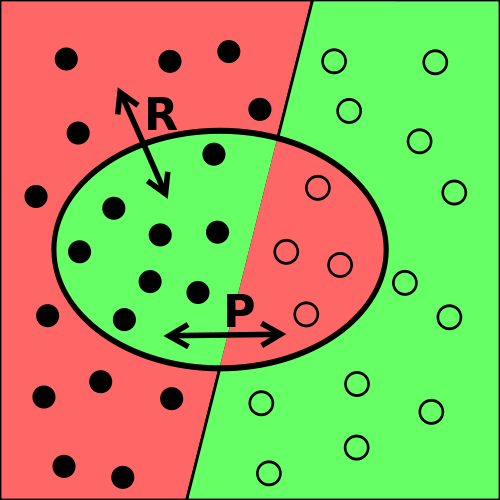
\includegraphics[width=0.5\textwidth]{recall-precision.png}
\label{fig:recall-precision}
\caption{Recall and precision example figure \cite{Wikipedia:Precision_and_recall}}
\end{figure}

\subsubsection{F-measure}
The \textit{F-measure} (F), or  balanced F-score or $\textit{F}_\textit{1}$ score, ...

\begin{figure}[H]
\begin{displaymath}
	\textit{F}_\textit{1} = 2 \cdot \frac{\pi \cdot \rho}{\pi + \rho}
\end{displaymath}
\caption{F-measure formula}
\end{figure}

\begin{figure}[H]
\begin{displaymath}
	\textit{F}_\beta = (1+\beta^2) \cdot \frac{\pi \cdot \rho}{(\beta^2 \cdot \pi) + \rho}
\end{displaymath}
\caption{General $\textit{F}_\beta$-score formula}
\end{figure}

$\textit{F}_\beta$ \enquote{measures the effectiveness of retrieval with respect to a user who attaches $\beta$ times as much importance to recall as precision} \cite{Rijsbergen:1979}.

\subsubsection{Error measure}
The \textit{error measure} (E) corresponds to the F-measure \cite{Feilmayr:2012}.

\begin{figure}[H]
\begin{displaymath}
	\textit{E} = 1 - \textit{F}_1
\end{displaymath}
\caption{Error measure formula}
\end{figure}

\subsubsection{Error Rate}
The \textit{Error Rate} (\textit{ERR}) ...

\begin{figure}[H]
\begin{displaymath}
	\textit{ERR} = \frac{S+D+I}{C+S+D+I}
\end{displaymath}
\caption{Error Rate formula}
\end{figure}

\subsubsection{Slot Error Rate}
The \textit{Slot Error Rate} (SER) ... 

\begin{figure}[H]
\begin{displaymath}
	SER = \frac{S+D+I}{N} = \frac{S+D+I}{C+S+D}
\end{displaymath}
\caption{Slot Error Rate formula}
\end{figure}

\subsection{Discussion}

\subsection{Runtime performance measures}

\subsubsection{CPU usage}
\subsubsection{Memory usage}